\chapter{Semantische Analyse} \label{chap:semantic}

Die semantische Analyse ist notwendig, da ein syntaktisch korrektes Programm logische Fehler beinhalten kann. Ein Beispiel dafür ist in \cref{lst:semantic-error} zu sehen. Darin wird eine Variable gelesen, bevor diese definiert wurde. Ein weiterer Fehler wäre es beispielsweise eine Funktion mit zu wenigen Parametern aufzurufen. Die Aufgabe der semantischen Analyse ist es, den erzeugten \ac{ast} zu durchlaufen und dabei die einzelnen Knoten auf solche Fehler zu prüfen.

\begin{lstlisting}[language=c, caption=Beispiel für einen semantischen Fehler, label={lst:semantic-error}]
	var r0 := r1;
	var r1 := 2;
\end{lstlisting}

\section{Abbilden auf eine Datenstruktur}
Um logische Fehler zu erkennen bietet es sich an eine eigene Datenstruktur zu entwerfen, welche das Programm abbildet und beim Durchlaufen des \ac{ast} diese Datenstruktur zu füllen. So kann, beispielsweise bei einem Funktionsaufruf, in der Datenstruktur nachgesehen werden, ob die entsprechende Funktion bereits deklariert wurde oder noch nicht. Ein weiterer Vorteil davon eine solche Datenstruktur zu definieren ist es, dass nach dem erfolgreichen Befüllen die Datenstruktur ausschließlich ein syntaktisch und semantisch korrektes Programm abbildet. Es wäre denkbar, die erzeugte Datenstruktur in einem nächsten Schritt anhand der gesammelten Daten zu optimieren und beispielsweise unbenutzte Funktionen zu entfernen, dies geschieht im aktuellen Stand der Arbeit nicht. 

In \cref{pic:Semantic-Struct} ist zu sehen, wie ein While-Programm auf eine Java-Klasse abgebildet wird. Knoten aus dem \ac{ast}, welche nicht relevant für die semantische Überprüfung oder die Codegenerierung sind, wie beispielsweise Semikolon oder Klammern werden nicht in die Datenstruktur mit aufgenommen, sondern ausschließlich Daten wie  Variablennamen, Werte einer Zuweisung, Name, Funktionsnamen und Funktionsparametern.

\begin{figure}[h!]
	%\includegraphics[width=1\textwidth]{content/pictures/LoRaWAN-OSI.JPG}
	\centering
	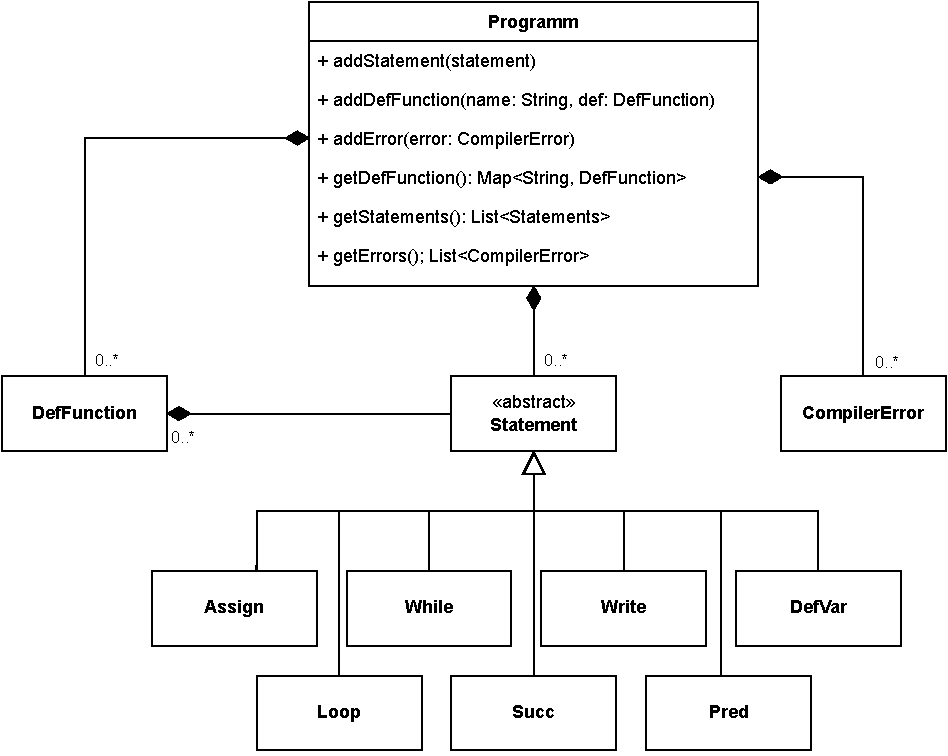
\includegraphics[width=13cm]{content/pictures/ClassDia.pdf}
	\caption{Ausschnitt der Datenstruktur}
	%	\source{\cite[S. 5]{SemtechCorporation.2020}}
	\label{pic:Semantic-Struct}
\end{figure}

\section{Durchlaufen des \acl{ast}}
Wie in \cref{subsec:antlr} bereits erklärt, wurde sich für diese Arbeit für den Visitor-Ansatz entschieden um den \ac{ast} zu durchlaufen. \ac{antlr} erzeugt beim Visitor-Ansatz eine \enquote{BaseVisitor}-Klasse. Diese beinhaltet für jeden Knoten eine Visit-Methode mit einem Parameter, welcher Informationen zum aktuellem Knoten enthält. Zusätzlich dazu ist die Methode in der Lage einen beliebigen Datentypen zurück zu geben. In \cref{lst:parser-basevisitor} ist der Inhalt der BaseVisitor-Klasse zu sehen.

\begin{lstlisting}[language=java, caption=Inhalt der generierten BaseVisitor-Klasse, label={lst:parser-basevisitor}]
	public class WhileBaseVisitor<T> extends ... {
		@Override public T visitProg(ProgContext ctx) { return visitChildren(ctx); }
		@Override public T visitRead(ReadContext ctx) { return visitChildren(ctx); }
		...
	}
\end{lstlisting}

In dieser Arbeit wurde für jeden Knoten eine Visitor-Klasse erstellt, welche von der Visitor-Baseklasse erbt und die entsprechende Visit-Methode implementiert. Zusätzlich dazu hat jede Visitor-Klasse eine Referenz zum Programm, so dass auf bereits definierte Strukturen zugriffen oder eine Fehlermeldung hinzugefügt werden kann. Mithilfe der Informationen aus dem Parameter können mit einer dazugehörigen Visitor-Klasse wiederum die Unterknoten durchlaufenen werden, beispielsweise die Statements innerhalb eines Funktionsdefinitionsknotens. Jede Visit-Methode gibt zum Schluss eine Instanz der entsprechenden Datenstruktur zurück.

In \cref{lst:semantic-deffunction} ist exemplarisch dargestellt, wie die Visitorklasse für Funktionsdefinitionsknoten aufgebaut ist. Darin ist zu sehen wie auf Unterknoten zugegriffen und zum Schluss ein Objekt zurück gegeben wird. Die Klasse \enquote{ProgramVisitor} nutzt die \enquote{DefFunctionVisitor}-Klasse um DefFunction-Knoten zu durchlaufen und erhält bei Erfolg ein DefFunction Objekt zurück, welches die \enquote{Program}-Klasse in ihrer Collection speichern kann.

\begin{lstlisting}[language=java, caption=Prinzipieller Aufbau einer Visitorklasse, label={lst:semantic-deffunction}]
	public class DefFunctionVisitor extends WhileBaseVisitor<DefFunction> {
		
		private Program program;
		
		public DefFunctionVisitor(Program program) {
			this.program = program;
		}
		
		@Override
		public DefFunction visitDefFunction(DefFunctionContext ctx) {
			 // Greife auf den Knoten ID zu
			Token nodeId = ctx.ID().getSymbol();
			
			// Greife auf die Parameter zu
			List<TerminalNode> functionParameters = ctx.defParameters().ID();
			
			// Greife auf die Statements der Funktion zu
			List<StatementContext> functionStatements = ctx.statement(); 
			
			// Greife auf bereits existierende Funktionen zu
			Map<String,DefFunction> def = program.getDefFunctions();
			
			// Fuehre Pruefungen durch
			// ....
			// Fuege eine Fehlermeldung dem Programm hinzu 
			 // program.addError(...);
			
			// Durchlaufe die Statement Knoten
			AvailableVariables availableVariables = new AvailableVariables();
			StatementVisitor statementVisitor = new StatementVisitor(availableVariables, programm);
			
			for (var statement : functionStatements) {
				Statement stmt = statement.accept(statementVisitor);
				if (stmt != null) {
					statements.add(stmt);
				}
			}
			// Gebe bei Erfolg ein Objekt zurueck, welches die Funktion abbildet
			return new DefDunction(nodeId, parameters, statements)
		}
\end{lstlisting}

\section{Prüfungen}
Wie in \cref{lst:semantic-deffunction} zu sehen ist, werden innerhalb der Visitor-Klassen, das heißt während des durchlaufen des Baums, auch die eigentlichen semantischen Prüfungen durchgeführt. Dabei handelt es sich um eine Menge von (verschachtelten) If-Abfragen. Die größte Menge an Prüfungen befindet sich im \enquote{DefFunctionVisitor} 
